\recipe{Sourdough}
\label{recipe:sourdough}
\makes{2 loaves}
\worktime{1 day}
\totaltime{2 days}
\source{}

\begin{ingredients}
\ingroup{Levain}
	\item 38 grams stoneground whole wheat flour
	\item 38 grams bread flour
	\item 76 grams water
	\item 38 grams ripe sourdough starter
\ingroup{Main dough}
	\item 773 grams bread flour
	\item 114 grams whole wheat flour
	\item 51 grams whole grain rye flour
	\item 653 grams water
	\item 18 grams fine sea salt
\end{ingredients}

\begin{method}

Levain (8:00 a.m.) Mix the levain ingredients and keep at 74-76°F (23-24°C) for 5 to 6 hours.

Autolyse (12:00 p.m) In a medium mixing bowl, mix the flour and 603 grams of water (reserve 50 grams until
the next step). Cover and let rest for 1 hour.

Mix (1:00 p.m.) To the mixing bowl holding your dough, add the salt, ripe levain (from step 1), and reserved 50
grams water. Mix by hand or with a dough whisk until incorporated. Transfer your dough to a bulk fermentation
container and cover.

Bulk Fermentation (1:10 p.m. to 5:10 p.m) Give the dough 3 sets of stretch and folds at 30-minute intervals,
where the first set starts 30 minutes after the start of bulk fermentation.

Divide and Preshape (5:10 p.m.) Lightly flour your work surface and scrape out your dough. Using your bench
knife, divide the dough in half. Lightly shape each half into a round shape. Let the dough rest for 25 minutes,
uncovered.

Shape (5:35 p.m.) Shape the dough into a round (boule) or oval (batard)—place in proofing baskets.

Rest and Proof (5:40 p.m. to 9:30 a.m. the next day) Cover proofing baskets with reusable plastic and seal
shut. Let the dough sit out on the counter for 20 minutes. Then, place both baskets into the refrigerator and proof
overnight.

Bake (Preheat oven at 8:30 a.m., bake at 9:30 a.m.) Preheat your oven with a combo cooker or Dutch oven
inside to 450°F (230°C). When the oven is preheated, remove your dough from the fridge, score it, and transfer
to the preheated combo cooker. Place the cooker in the oven, cover with the lid, and bake for 20 minutes. After
this time, remove the lid (you can keep it in the oven or remove it) and continue to bake for 30 minutes longer.
When done, the internal temperature should be around 208°F (97°C). Let the loaves cool for 1 to 2 hours on a
wire rack before slicing.
\end{method}




\begin{figure}[h]
  	\centering
  	
  	\begin{tikzpicture}
  		% Save the image in a box to get its dimensions
  		\sbox0{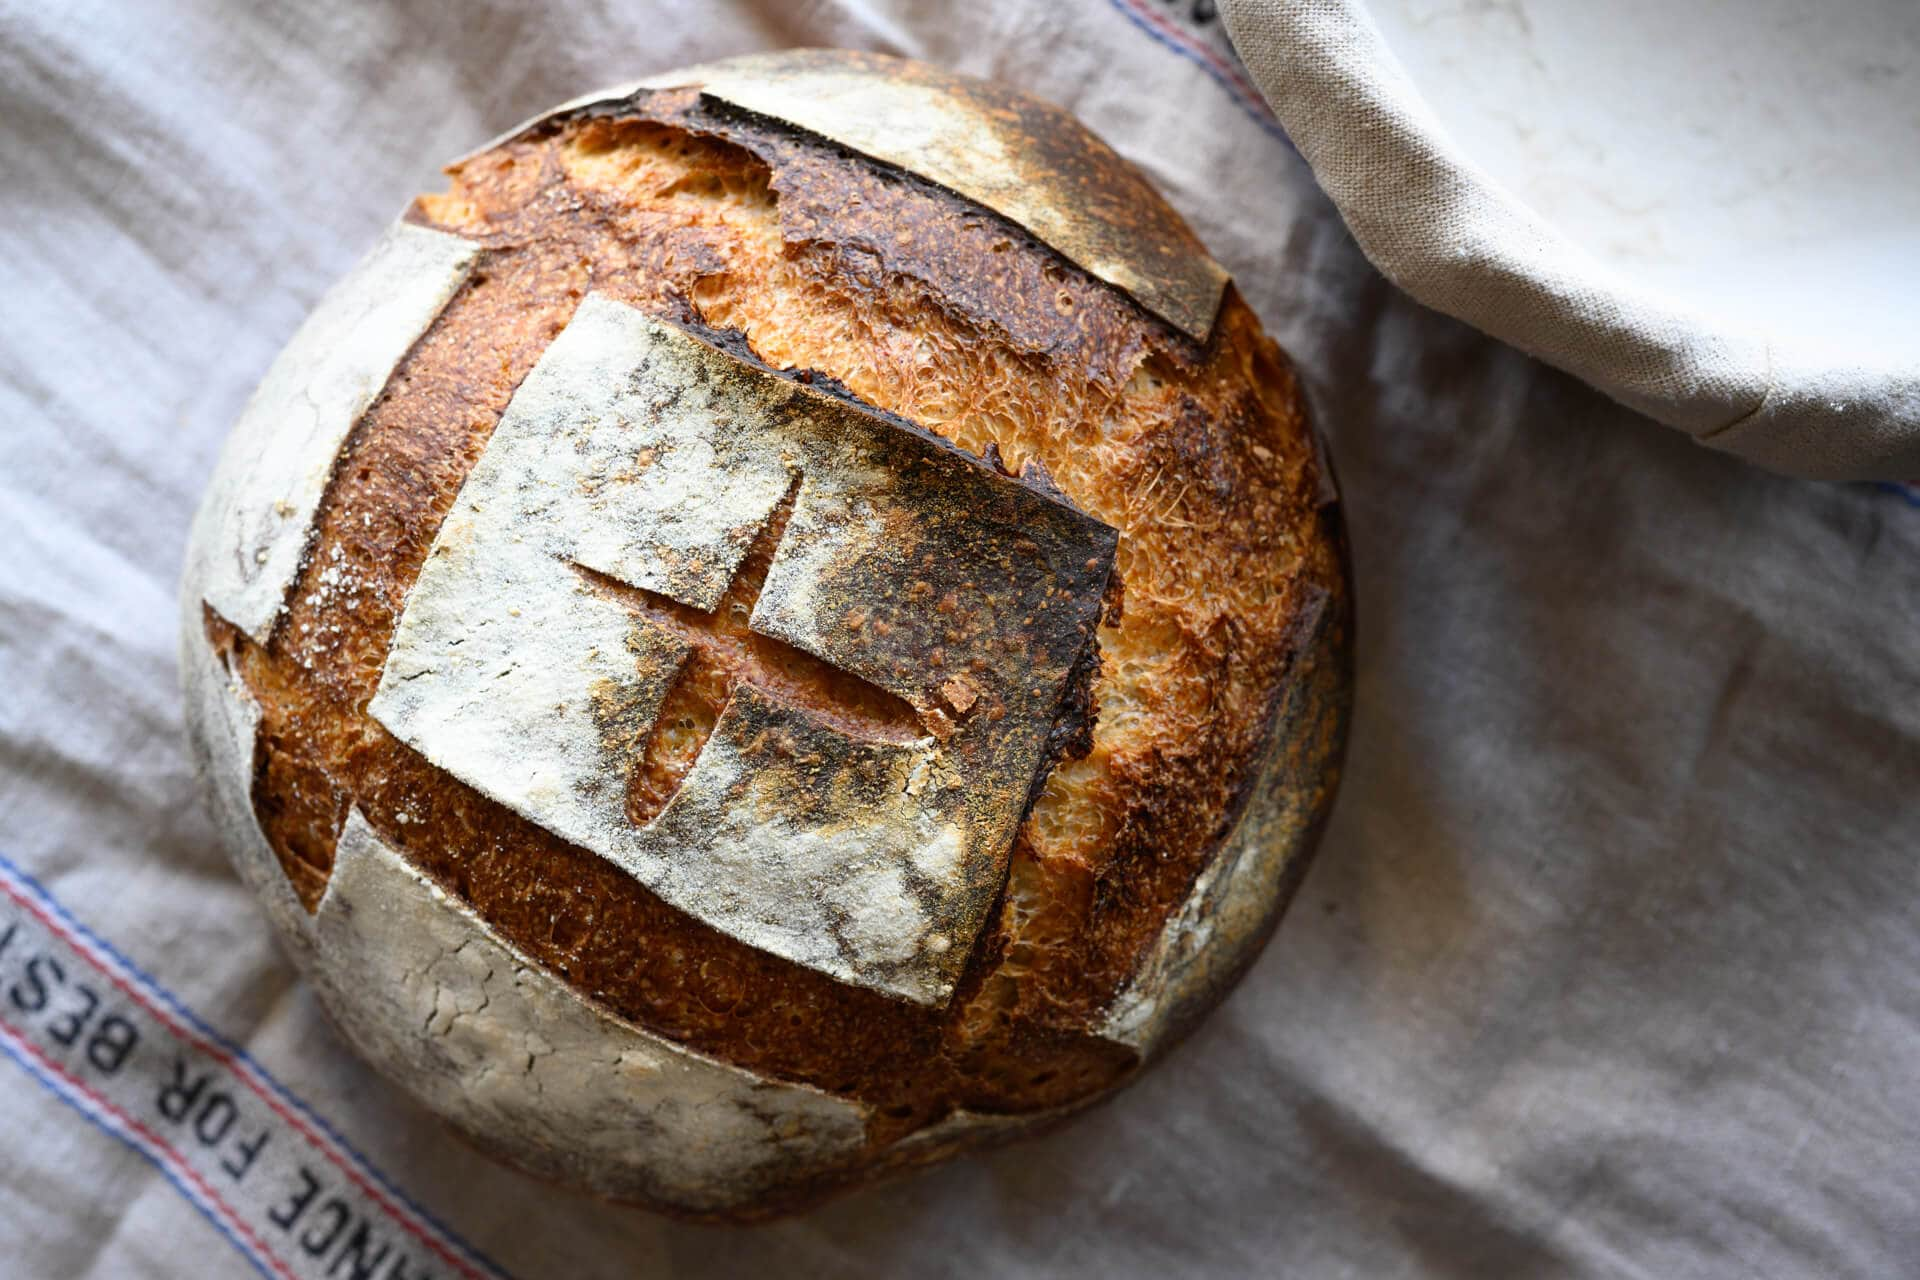
\includegraphics[width=\linewidth]{images/theperfectloaf-a-simple-workweek-sourdough-bread-recipe-1.jpg}}%
  
  		% Draw a clipping rectangle with rounded corners
  		\path[clip, rounded corners=0.5cm] (0,0) rectangle (\wd0,\ht0);
  
  		% Place the image inside the clipped area
  		\node[inner sep=0pt, outer sep=0pt, anchor=south west] at (0,0) {\usebox0};
	\end{tikzpicture}

  \caption*{}
\end{figure}
    
